\bookchapter{第六十章：搭建开发环境——Xcode 与第一个项目}

\chapterintro{工欲善其事，必先利其器。这一章咱们把“厨房”搭好：装好 Xcode、跑通模拟器、创建人生第一个 iOS 项目，再把工程结构拆开看个明白。装好环境之后，你会第一次看到自己写的代码变成一个能点的按钮——这个瞬间，很多人会记一辈子。}

\booksection{一、准备一台 Mac}

先说门槛：iOS 开发必须在 macOS 上进行。如果你没有 Mac，选项有三：买一台（哪怕是二手 Mac mini 或 MacBook Air 都够用）、短期租云 Mac、或者先读第八篇《安卓开发实战篇》（Windows 就能干）。

\begin{center}
\begin{tabularx}{\linewidth}{|X|X|X|}
\hline
\textbf{配置项} & \textbf{最低要求} & \textbf{舒适线（推荐）} \tabularnewline
\hline
芯片 & Apple Silicon（M1 起） & M2 及更新 \tabularnewline
内存 & 8GB & 16GB \tabularnewline
磁盘 & 预留 40GB+（Xcode 本体很胖） & 256GB 起步 \tabularnewline
系统 & 最新 macOS & 保持自动更新 \tabularnewline
\hline
\end{tabularx}
\end{center}

\begin{center}\small\color{gray}Mac 开发机配置参考（2026 年 8 月）\end{center}

\begin{tcbinfo}{小贴士：没有 Mac 也能先学语言}
iPad 上免费的\textbf{Swift Playgrounds}能学 Swift 语言基础（不用 Mac）；甚至 iPhone 上也能装。先把第 61 章的语言知识在 Playgrounds 里玩熟，等拿到 Mac 后直接起飞。磨刀不误砍柴工，说的就是这个。

\end{tcbinfo}

\booksection{二、安装 Xcode}

Xcode 是苹果官方的集成开发环境，免费。三步装好：

\begin{enumerate}
  \item Mac 上打开\textbf{App Store}，搜索 "Xcode"，点安装——注意它有好几个 GB，找个网速好的时段；
  \item 装完首次启动，同意协议、装完组件（自动完成）；
  \item 菜单 Xcode Settings Locations，确认\textbf{Command Line Tools}已选中——命令行工具是很多脚本和第三方工具的前提。
\end{enumerate}

\begin{tcbwarn}{注意：版本和系统的"匹配游戏"}
新 Xcode 往往要求最新 macOS，旧 Mac 则会卡在老版本。上架 App Store 时，苹果会要求用\textbf{较新的 Xcode}构建（通常给一个宽限期）。所以系统更新别拖太久——iOS 开发者是“追新版”最勤快的一群人。

\end{tcbwarn}

\booksection{三、创建你的第一个项目}

打开 XcodeCreate New Project选\textbf{iOS App}模板，然后填：

\begin{center}
\begin{tabularx}{\linewidth}{|X|X|X|}
\hline
\textbf{配置项} & \textbf{填什么} & \textbf{说明} \tabularnewline
\hline
Product Name & MyFirstApp & 应用名字 \tabularnewline
Team & 你的 Apple ID（免费） & 签名用，个人账号即可 \tabularnewline
Organization Identifier & com.example & 和 Product Name 拼成包标识 \tabularnewline
Interface & SwiftUI & 本书主线框架 \tabularnewline
Language & Swift & 不解释 \tabularnewline
\hline
\end{tabularx}
\end{center}

\begin{center}\small\color{gray}创建项目要填的五件事\end{center}

点 Create 后，Xcode 会生成一个能直接跑的项目。左上角选一台模拟器（比如 iPhone 17），点 > 运行——几秒后，模拟器屏幕上出现一个写着 “Hello, world!” 的窗口。\textbf{你的第一个 iOS App 已经诞生了}。

\booksection{四、工程结构拆解：每个文件是干嘛的}

左侧是工程导航器，新手只需认识这几个：

\begin{center}
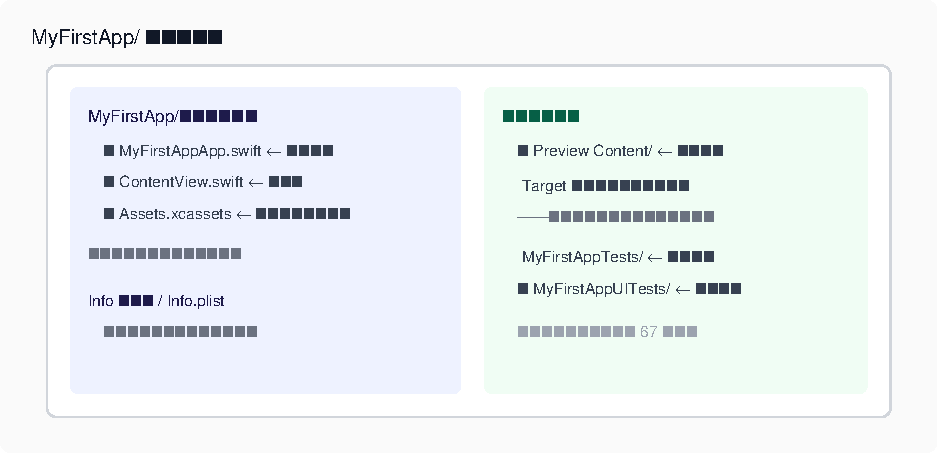
\includegraphics[width=0.92\linewidth]{figures/fig-di-liu-shi-zhang-1}
\\[2pt]\small 图 2：新手必懂的 Xcode 工程结构
\end{center}

\begin{itemize}
  \item \textbf{MyFirstAppApp.swift}：程序入口，SwiftUI 里它只有几行——"启动，然后显示主界面"；
  \item \textbf{ContentView.swift}：主界面视图，你现在看到的一切都在这里；
  \item \textbf{Assets.xcassets}：资源仓库——图标、图片、颜色都放这；
  \item \textbf{Target 设置}：点左侧蓝色工程图标进去，版本号、最低 iOS 版本、签名都在里面。App 显示名、图标也在这配置。
\end{itemize}

\booksection{五、真机调试：把 App 装进你的 iPhone}

\booksection{五、Xcode 效率技巧：新手的五个“快捷键外挂”}

用熟这几个，你会显得“很专业”：

\begin{center}
\begin{tabularx}{\linewidth}{|X|X|X|}
\hline
\textbf{操作} & \textbf{快捷键} & \textbf{作用} \tabularnewline
\hline
运行 & CmdR & 编译并跑起来 \tabularnewline
打开/切换画布预览 & OptionCmd & 所见即所得的开关 \tabularnewline
格式化缩进 & CtrlI & 自动整理选中代码的缩进 \tabularnewline
快速打开文件 & CmdO & 输入文件名秒开（最常用！） \tabularnewline
注释/取消注释 & Cmd/ & 调试时随手开关代码 \tabularnewline
\hline
\end{tabularx}
\end{center}

\begin{center}\small\color{gray}Xcode 高频快捷键（新手五件套）\end{center}

另外两个隐藏福利：\textbf{多开模拟器}（同时跑 iPhone 和 iPad 对比布局）和\textbf{代码片段库}（把常用的几行代码拖进右侧 Snippets 面板，下次一键插入）——效率工具先用起来，手感自然就上来了。

\booksection{六、真机调试：把 App 装进你的 iPhone}

模拟器虽好，真机才是终点。用免费 Apple ID 也能真机调试：

\begin{enumerate}
  \item 数据线连上 iPhone（或同 Wi-Fi 无线调试）；
  \item Xcode 顶部设备列表选你的手机，首次会提示登录 Apple ID 并自动配置签名；
  \item iPhone 上 [设置] [通用] [VPN与设备管理] 信任你的开发者证书；
  \item 点 >，App 装进真机。
\end{enumerate}

\begin{tcbwarn}{注意：免费账号的"七天限制"}
免费 Apple ID 签名的 App\textbf{7 天后会失效}（重新运行一次即可续期）。这是苹果的防滥用机制，学习阶段完全够用；付费开发者账号（99 美元/年）则没有这个限制，第 67 章细说。

\end{tcbwarn}

\booksection{七、小试牛刀 + 常见报错急救}

\booksection{六、小试牛刀 + 常见报错急救}

打开 ContentView.swift，把\texttt{Text(“Hello, world!”)}里的字换成你的名字，按CmdR重新运行——几秒后模拟器上就显示你的名字。恭喜，你完成了第一次完整的“改代码 编译 安装 运行”循环。

\begin{center}
\begin{tabularx}{\linewidth}{|X|X|X|}
\hline
\textbf{报错现象} & \textbf{常见原因} & \textbf{解药} \tabularnewline
\hline
Signing 报错 & Team 没选、证书过期 & Target Signing 里勾上你的账号；免费账号重跑一次 \tabularnewline
模拟器黑屏/打不开 & 镜像损坏 & 菜单 Device Erase All Content；或删掉重加模拟器 \tabularnewline
Xcode 下载慢/装不上 & App Store 网络波动 & 换时段；或到苹果开发者网站下载 .xip 离线包 \tabularnewline
\hline
\end{tabularx}
\end{center}

\begin{center}\small\color{gray}新手环境报错急救表\end{center}

\begin{tcbpractice}{来动手：完成你的"开发仪式感"清单}
(1) 装好 Xcode 并跑通模拟器；(2) 用真机跑一次自己的 App 并截图留念；(3) 把 Hello 文字改成你的名字；(4) 到 Target 设置里把 App 显示名改成“我的第一个App”。做完这四步，你就是有作品的人了。

\end{tcbpractice}

\begin{tcbsummary}{本章小结}
\begin{itemize}
  \item 硬门槛：Mac + Xcode；没有 Mac 先用 iPad 上的 Swift Playgrounds 学语言
  \item Xcode 从 App Store 装；新版本要求新系统，更新别拖
  \item 新建项目五要素：名字、Team、组织标识、SwiftUI、Swift
  \item 工程口诀：代码都在 MyFirstApp/ 目录；Target 设置管版本与签名
  \item 免费 Apple ID 真机调试有 7 天签名限制；付费账号无此限制
  \item 开发日常 = 改代码 CmdR 看效果，循环往复
\end{itemize}

\end{tcbsummary}
